\chapter{Analyse fonctionnelle et conception du système}
\label{chap:analyse}

\section{Introduction}

Après avoir défini les objectifs, le périmètre et les contraintes du projet dans le cahier des charges, cette deuxième étape vise à analyser le \textbf{fonctionnement attendu du système} afin de poser les bases de sa conception. L'analyse fonctionnelle assure la cohérence entre les attentes du sujet et la structure technique de la solution. Dans un premier temps, nous identifierons les acteurs et les cas d'utilisation, puis nous décrirons les scénarios de démonstration. Nous formaliserons ensuite le comportement du système à travers les diagrammes \textbf{UML} de cas d'utilisation, d'activité, de séquence et de composants.

\section{Identification des acteurs}

L'identification des acteurs constitue une étape essentielle de l'analyse fonctionnelle. Elle permet de déterminer les différentes parties qui interagissent avec le système, chacune ayant un rôle et des responsabilités spécifiques.

\textbf{1. Équipe projet}\\
\textbf{Rôle :} l'équipe conçoit et entraîne le modèle de classification.\\
\textbf{Responsabilités :}
\begin{itemize}
  \item Préparer les données et réaliser leur découpage.
  \item Entraîner et comparer les classifieurs.
  \item Évaluer le modèle final et analyser ses erreurs.
\end{itemize}

\textbf{2. Utilisateur de la démonstration}\\
\textbf{Rôle :} l'utilisateur interagit avec le système pour observer son fonctionnement.\\
\textbf{Responsabilités :}
\begin{itemize}
  \item Classer une nouvelle image.
  \item Lancer un épisode de conduite dans le simulateur.
\end{itemize}

\textbf{3. Encadrante et jury}\\
\textbf{Rôle :} l'encadrante valide les choix du projet et suit son avancement, tandis que le jury évalue les résultats.\\
\textbf{Responsabilités :}
\begin{itemize}
  \item Valider le jeu de données et le périmètre du projet.
  \item Consulter les résultats, le rapport et la démonstration.
\end{itemize}

À ces acteurs humains s'ajoutent deux acteurs système : le \textbf{simulateur}, qui fournit l'environnement, les positions des objets et leurs images, et le \textbf{modèle ML}, qui renvoie la classe et le score d'une image.

\begin{table}[H]
\centering
\caption{Résumé des acteurs et de leurs rôles}
\begin{tabularx}{\textwidth}{>{\raggedright\arraybackslash}p{3.6cm}>{\raggedright\arraybackslash}p{2.2cm}Y}
  \toprule
  \entete \textbf{Acteur} & \textbf{Type} & \textbf{Rôle principal} \\
  \midrule
  Équipe projet & Humain & Préparation des données, entraînement et évaluation des modèles \\
  Utilisateur de la démo & Humain & Classification d'images et lancement d'épisodes de conduite \\
  Encadrante & Humain & Validation des choix et suivi de l'avancement \\
  Jury & Humain & Évaluation des résultats, du rapport et de la démonstration \\
  Simulateur & Système & Environnement, positions et images des objets \\
  Modèle ML & Système & Classe et score de chaque image \\
  \bottomrule
\end{tabularx}
\end{table}

\section{Description des cas d'utilisation}

\begin{table}[H]
\centering
\small
\caption{Description des cas d'utilisation}
\begin{tabularx}{\textwidth}{l>{\raggedright\arraybackslash}p{3.6cm}>{\raggedright\arraybackslash}p{2.4cm}Y}
  \toprule
  \entete \textbf{ID} & \textbf{Cas d'utilisation} & \textbf{Acteur} & \textbf{Résultat attendu} \\
  \midrule
  UC1 & Préparer les données & Équipe & Recadrages filtrés, normalisés et découpés en entraînement, validation et test \\
  UC2 & Entraîner et comparer les classifieurs & Équipe & Tableau comparatif de SVM, Random Forest et k-NN sur la validation \\
  UC3 & Évaluer le modèle final & Équipe, encadrante & Scores sur le test, matrice de confusion et analyse des erreurs \\
  UC4 & Classer une nouvelle image & Utilisateur & \og photo.jpg \textrightarrow{} Voiture (92~\%) \fg{} \\
  UC5 & Lancer une démonstration de conduite & Utilisateur, jury & Le véhicule rejoint sa destination en réagissant aux obstacles \\
  UC6 & Comparer les classifieurs dans le simulateur & Équipe & Collisions, fautes graves et décisions inadaptées sur plusieurs épisodes \\
  UC7 & Consulter les résultats et le rapport & Encadrante, jury & Notebooks commentés, figures et rapport \\
  \bottomrule
\end{tabularx}
\end{table}

\section{Scénarios de fonctionnement}
\label{sec:scenarios}

Ces scénarios serviront à la fois à concevoir les tests et à montrer ce que le système final devra accomplir. Les illustrations de la figure~\ref{fig:scenarios} proviennent d'autres simulateurs et servent uniquement d'inspiration. Une capture de notre propre simulateur est présentée à la section~\ref{sec:environnement}.

\begin{figure}[H]
  \centering
  \begin{subfigure}[t]{0.48\textwidth}
    \centering
    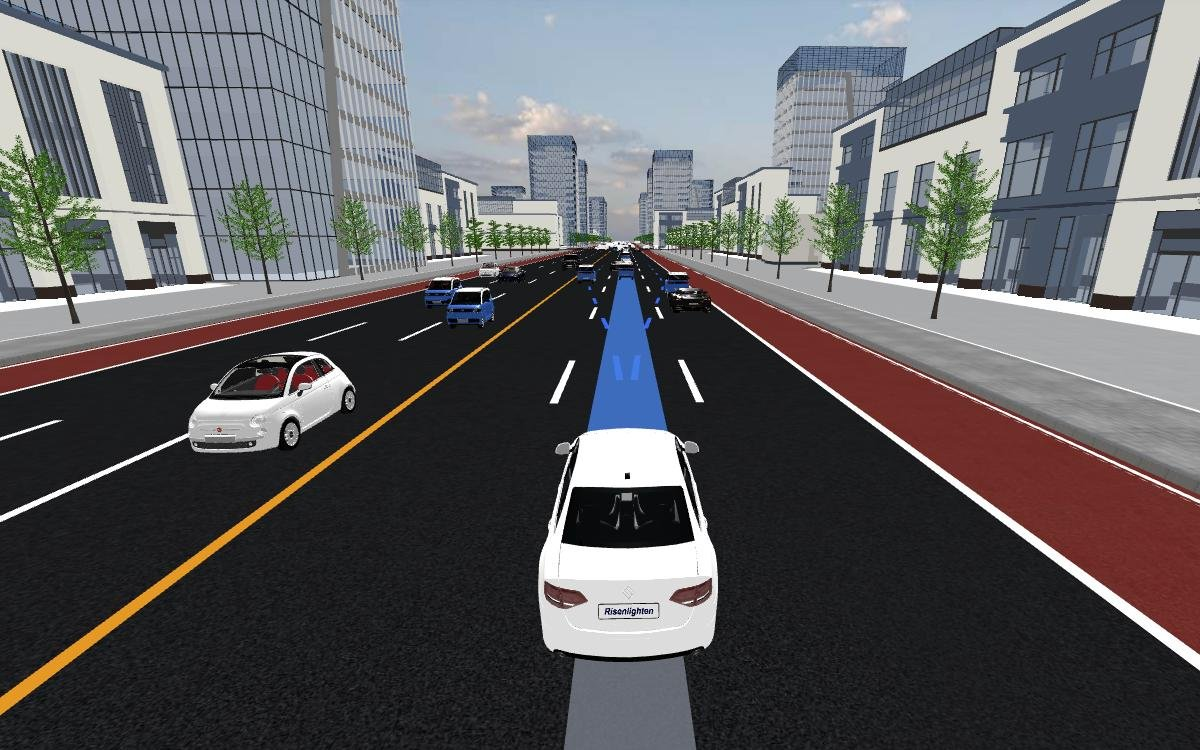
\includegraphics[width=\textwidth,height=4.2cm,keepaspectratio]{scenario1route_libre.jpg}
    \caption{Scénario 1 : route libre}
  \end{subfigure}\hfill
  \begin{subfigure}[t]{0.48\textwidth}
    \centering
    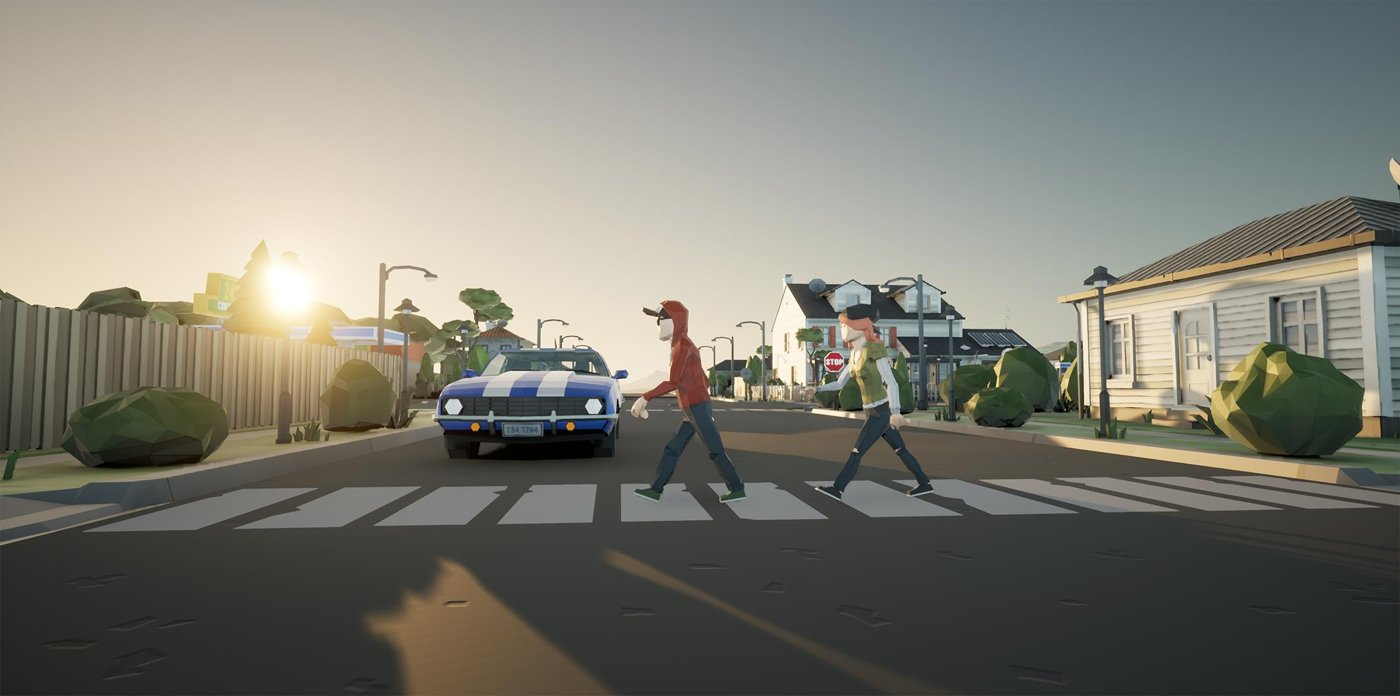
\includegraphics[width=\textwidth,height=4.2cm,keepaspectratio]{scenario2_presence_pieton.jpg}
    \caption{Scénario 2 : présence d'un piéton}
  \end{subfigure}

  \vspace{0.6em}
  \begin{subfigure}[t]{0.48\textwidth}
    \centering
    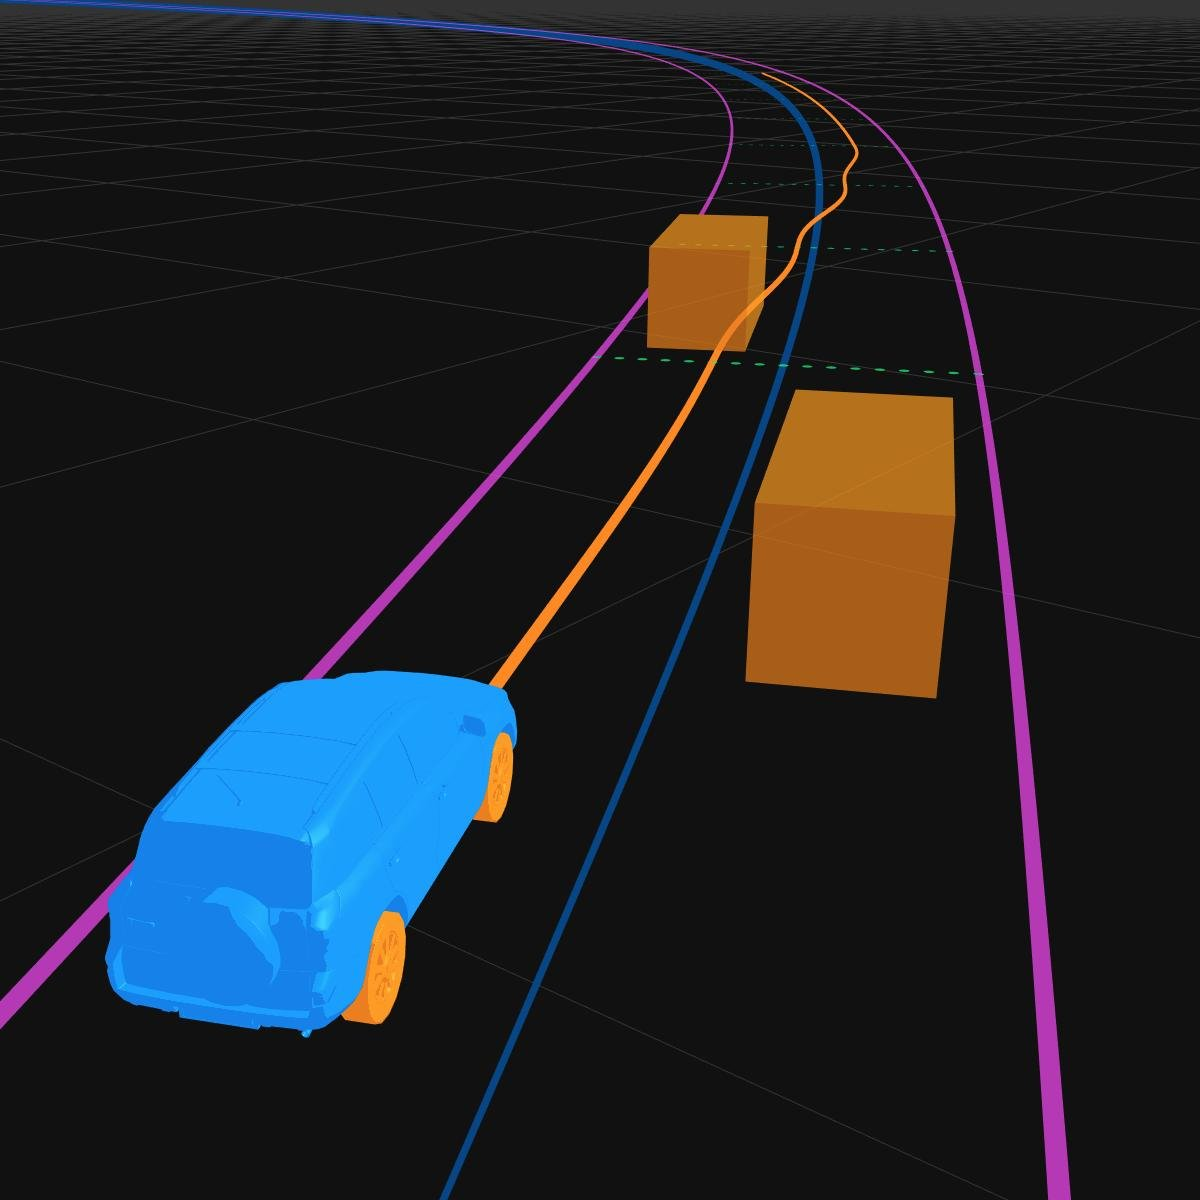
\includegraphics[width=\textwidth,height=4.6cm,keepaspectratio]{scenario3route_bloquee.jpg}
    \caption{Scénario 3 : route bloquée}
  \end{subfigure}\hfill
  \begin{subfigure}[t]{0.48\textwidth}
    \centering
    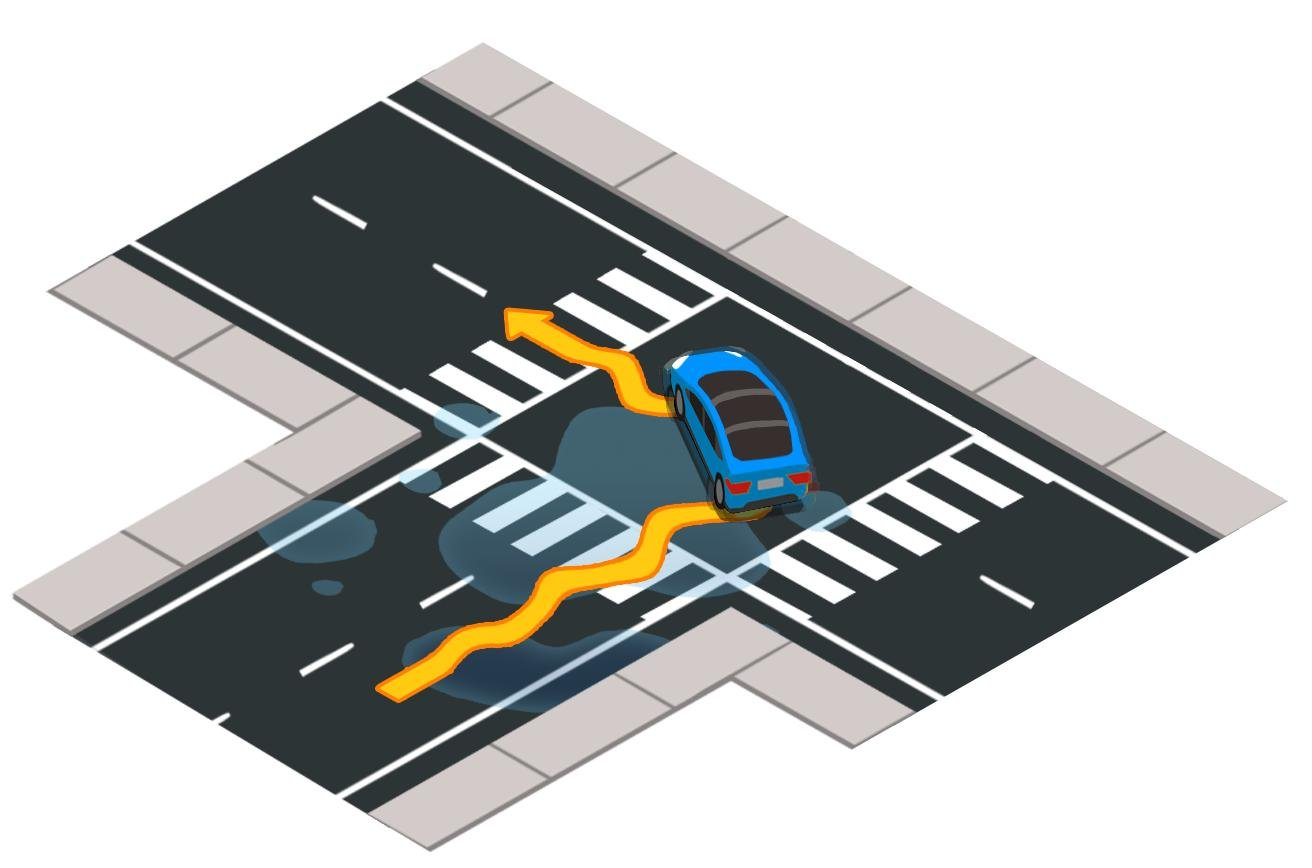
\includegraphics[width=\textwidth,height=4.6cm,keepaspectratio]{scenario4contournement.jpg}
    \caption{Scénario 4 : contournement}
  \end{subfigure}
  \caption{Scénarios de démonstration (illustrations externes)}
  \label{fig:scenarios}
\end{figure}

\begin{itemize}
  \item \textbf{Scénario 1 : route libre (cas nominal)}\\
  Aucun obstacle ne se trouve sur l'itinéraire. Le véhicule suit le chemin calculé par Dijkstra jusqu'à sa destination.
  \item \textbf{Scénario 2 : présence d'un piéton}\\
  Un objet classé \og personne \fg{} se trouve sur l'itinéraire, à moins de 35~m. Le véhicule s'arrête, attend que la personne traverse, puis repart sur le même trajet.
  \item \textbf{Scénario 3 : route bloquée}\\
  Un objet classé \og voiture \fg{}, \og bus \fg{} ou \og camion \fg{} occupe le tronçon. Celui-ci est marqué comme bloqué dans le graphe, et Dijkstra recherche un autre chemin.
  \item \textbf{Scénario 4 : contournement}\\
  Un nouveau chemin existe. Le véhicule change de rue, ou fait demi-tour si nécessaire, puis reprend sa progression vers la destination.
\end{itemize}

Deux cas particuliers sont également prévus. Si le score de confiance est trop faible, la classe devient \og Inconnu \fg{} et le véhicule effectue un arrêt prudent. S'il n'existe plus aucun chemin, le véhicule reste arrêté, et l'épisode est déclaré \og bloqué \fg{} au bout de 30 pas.

\section{Diagramme de cas d'utilisation}

Le diagramme de cas d'utilisation du projet \textit{AutoMaze AI} illustre les différentes interactions entre les acteurs et les fonctionnalités principales du système. L'équipe projet intervient sur toute la chaîne de Machine Learning, de la préparation des données à l'évaluation. L'utilisateur de la démonstration peut classer une image ou lancer un épisode de conduite, tandis que l'encadrante et le jury consultent les résultats. Le diagramme met également en évidence le lien d'\textbf{inclusion} entre la démonstration de conduite et la classification d'une image, puisque chaque obstacle rencontré doit être classé.

\begin{figure}[H]
  \centering
  \resizebox{\textwidth}{!}{% Diagramme de cas d'utilisation : acteurs à gauche et à droite, cas d'utilisation dans le système
\begin{tikzpicture}[
    uc/.style={ellipse, draw=accent, fill=accent!7, align=center, font=\footnotesize,
               minimum width=4.1cm, minimum height=0.95cm, inner sep=1pt},
    lien/.style={draw=black!60},
    inclut/.style={draw=black!50, dashed, -{Stealth[length=2mm]}}
  ]
  % Bonhomme : \acteur{nom}{position}{texte}
  \newcommand{\acteur}[3]{
    \begin{scope}[shift={#2}]
      \draw[thick] (0,0.55) circle (0.17);
      \draw[thick] (0,0.38) -- (0,-0.12);
      \draw[thick] (-0.3,0.2) -- (0.3,0.2);
      \draw[thick] (0,-0.12) -- (-0.22,-0.5);
      \draw[thick] (0,-0.12) -- (0.22,-0.5);
      \node[font=\footnotesize, align=center] at (0,-0.85) {#3};
      \coordinate (#1) at (0,0.1);
    \end{scope}
  }

  % Système
  \draw[draw=black!55, rounded corners=4pt] (2.2,0.9) rectangle (11.4,-8.6);
  \node[anchor=north west, font=\small\bfseries] at (2.3,0.85) {Système AutoMaze AI};

  \node[uc] (u1) at (6.8,-0.4) {UC1 Préparer les données};
  \node[uc] (u2) at (6.8,-1.65) {UC2 Entraîner et comparer\\les classifieurs};
  \node[uc] (u3) at (6.8,-2.9) {UC3 Évaluer le modèle final};
  \node[uc] (u4) at (6.8,-4.15) {UC4 Classer une nouvelle image};
  \node[uc] (u5) at (6.8,-5.4) {UC5 Lancer une démonstration\\de conduite};
  \node[uc] (u6) at (6.8,-6.65) {UC6 Comparer les classifieurs\\dans le simulateur};
  \node[uc] (u7) at (6.8,-7.9) {UC7 Consulter les résultats\\et le rapport};

  \acteur{equipe}{(0,-1.6)}{Équipe\\projet}
  \acteur{utilisateur}{(0,-5.6)}{Utilisateur\\de la démo}
  \acteur{encadrant}{(13.6,-3.2)}{Encadrant}
  \acteur{jury}{(13.6,-6.7)}{Jury}

  \foreach \u in {u1,u2,u3,u6} \draw[lien] (equipe) -- (\u.west);
  \foreach \u in {u4,u5} \draw[lien] (utilisateur) -- (\u.west);
  \draw[lien] (encadrant) -- (u7.east);
  \draw[lien] (encadrant) -- (u3.east);
  \draw[lien] (jury) -- (u7.east);
  \draw[lien] (jury) -- (u5.east);

  % Le cas UC5 inclut la classification d'une image
  \draw[inclut] (u5.north east) to[bend right=30] node[right, font=\scriptsize, text=black!60] {« inclut »} (u4.south east);
\end{tikzpicture}
}
  \caption{Diagramme de cas d'utilisation}
\end{figure}

\section{Diagramme d'activité}

Le diagramme d'activité décrit le déroulement d'un \textbf{épisode de conduite}, depuis le calcul de l'itinéraire jusqu'à l'arrivée. À chaque pas, le véhicule avance puis vérifie s'il a atteint sa destination. Lorsqu'un obstacle se trouve à moins de 35~m, son image est transmise au modèle, et la classe prédite détermine l'action à appliquer. Les coûts des tronçons sont alors mis à jour, et le trajet est recalculé. Ce diagramme met en évidence la coordination entre la perception, la décision et la planification.

\begin{figure}[H]
  \centering
  \resizebox{0.95\textwidth}{!}{% Diagramme d'activité : déroulement d'un épisode de conduite dans le simulateur
\begin{tikzpicture}[
    node distance=0.42cm,
    act/.style={draw=accent, fill=accent!7, rounded corners=6pt, align=center, font=\footnotesize,
                text width=5.4cm, minimum height=0.75cm},
    choix/.style={diamond, draw=black!60, fill=white, aspect=2.4, align=center, font=\scriptsize,
                  inner sep=1pt, text width=2.2cm},
    fleche/.style={-{Stealth[length=2mm]}, draw=black!65, thick}
  ]
  \node[circle, fill=black, minimum size=0.35cm] (debut) {};
  \node[act, below=of debut] (route) {Calculer l'itinéraire avec Dijkstra};
  \node[act, below=of route] (avance) {Avancer d'un pas sur l'itinéraire};
  \node[choix, below=of avance] (arrive) {Destination atteinte ?};
  \node[choix, below=0.5cm of arrive] (obstacle) {Obstacle à moins de 35~m ?};
  \node[act, below=0.5cm of obstacle] (image) {Recevoir l'image de l'obstacle (caméra virtuelle)};
  \node[act, below=of image] (classe) {Classer l'image : classe et score};
  \node[choix, below=of classe] (seuil) {Score au-dessus du seuil ?};
  \node[act, below=0.5cm of seuil] (decision) {Choisir l'action selon la classe prédite};
  \node[act, below=of decision] (couts) {Mettre à jour les coûts des tronçons et recalculer le trajet};
  \node[choix, below=of couts] (chemin) {Un chemin existe ?};

  \node[act, right=1.3cm of seuil] (inconnu) {« Inconnu » : arrêt prudent};
  \node[act, left=1.3cm of chemin] (attente) {Attendre (au plus 30 pas), puis épisode « bloqué »};
  \node[circle, draw=black, thick, minimum size=0.45cm, right=1.3cm of arrive] (fin) {};
  \node[circle, fill=black, minimum size=0.25cm] at (fin) {};

  \draw[fleche] (debut) -- (route);
  \draw[fleche] (route) -- (avance);
  \draw[fleche] (avance) -- (arrive);
  \draw[fleche] (arrive) -- node[above, font=\scriptsize] {oui} (fin);
  \draw[fleche] (arrive) -- node[right, font=\scriptsize] {non} (obstacle);
  \draw[fleche] (obstacle) -- node[right, font=\scriptsize] {oui} (image);
  \draw[fleche] (obstacle.west) -- ++(-1.2,0) node[above, font=\scriptsize, pos=0.4] {non} |- (avance.west);
  \draw[fleche] (image) -- (classe);
  \draw[fleche] (classe) -- (seuil);
  \draw[fleche] (seuil) -- node[right, font=\scriptsize] {oui} (decision);
  \draw[fleche] (seuil) -- node[above, font=\scriptsize] {non} (inconnu);
  \draw[fleche] (inconnu) |- (couts);
  \draw[fleche] (decision) -- (couts);
  \draw[fleche] (couts) -- (chemin);
  \draw[fleche] (chemin.east) -- ++(3.4,0) node[above, font=\scriptsize, pos=0.25] {oui} |- (avance.east);
  \draw[fleche] (chemin) -- node[above, font=\scriptsize] {non} (attente);
\end{tikzpicture}
}
  \caption{Diagramme d'activité d'un épisode de conduite}
\end{figure}

\section{Diagramme de séquence}

Le diagramme de séquence décrit les échanges entre les modules lorsque le véhicule rencontre un obstacle. Le moteur de simulation demande l'image de l'obstacle à la caméra virtuelle, puis la transmet au classifieur, qui renvoie la classe, le score et les six probabilités. La classe prédite et la position de l'obstacle sont ensuite envoyées au système de décision, qui modifie le graphe, avant que le planificateur ne recalcule le trajet. Il est important de noter que la \textbf{vraie classe de l'objet n'apparaît dans aucun message} : le système de décision ne reçoit que la classe prédite.

\begin{figure}[H]
  \centering
  \resizebox{\textwidth}{!}{% Diagramme de séquence : traitement d'un obstacle détecté par le véhicule
\begin{tikzpicture}[
    tete/.style={draw=accent, fill=accent!7, rounded corners=2pt, font=\footnotesize, align=center,
                 minimum width=2.15cm, minimum height=0.8cm},
    msg/.style={-{Stealth[length=2mm]}, draw=black!75},
    retour/.style={-{Stealth[length=2mm]}, draw=black!60, dashed},
    texte/.style={font=\scriptsize, above, align=center}
  ]
  % Lignes de vie : nom, abscisse
  \foreach \nom/\x/\titre in {moteur/0/Moteur\\de simulation, camera/2.6/Caméra\\virtuelle, modele/5.2/Classifieur\\(modèle ML),
                              decision/7.8/Système\\de décision, plan/10.4/Planificateur\\(Dijkstra), vehicule/13/Contrôleur\\du véhicule} {
    \node[tete] (\nom) at (\x,0) {\titre};
    \draw[black!40, dashed] (\x,-0.45) -- (\x,-9.4);
  }

  \draw[msg] (0,-1.2) -- node[texte] {image(obstacle)} (2.6,-1.2);
  \draw[retour] (2.6,-1.8) -- node[texte] {image RGB} (0,-1.8);
  \draw[msg] (0,-2.6) -- node[texte, pos=0.5] {predict(image)} (5.2,-2.6);
  \draw[retour] (5.2,-3.3) -- node[texte, pos=0.5] {classe, score, 6 probabilités} (0,-3.3);
  \draw[msg] (0,-4.1) -- node[texte, pos=0.62] {classe prédite + position de l'obstacle} (7.8,-4.1);
  \draw[msg] (7.8,-4.9) -- node[texte] {bloquer ou pénaliser\\le tronçon} (10.4,-4.9);
  \draw[msg] (10.4,-5.9) -- ++(0.55,0) -- ++(0,-0.45) -- ++(-0.55,0);
  \node[font=\scriptsize, anchor=west, align=left] at (11.05,-6.1) {recalcul\\du trajet};
  \draw[retour] (10.4,-6.9) -- node[texte] {nouvel itinéraire} (7.8,-6.9);
  \draw[msg] (7.8,-7.7) -- node[texte, pos=0.5] {action : arrêter, ralentir, contourner} (13,-7.7);
  \draw[retour] (13,-8.6) -- node[texte, pos=0.5] {nouvelle position du véhicule} (0,-8.6);

  % Activation du classifieur
  \fill[accent!25] (5.1,-2.6) rectangle (5.3,-3.3);
\end{tikzpicture}
}
  \caption{Diagramme de séquence du traitement d'un obstacle}
\end{figure}

\section{Diagramme de composants}

Le diagramme de composants présente l'organisation logicielle du projet. La chaîne de Machine Learning, réalisée dans les notebooks, produit les poids du modèle et le fichier \texttt{metadata.json}. Le simulateur charge ces fichiers à travers son module de perception, et les différents modules communiquent grâce aux contrats partagés définis dans \texttt{contracts.py}.

\begin{figure}[H]
  \centering
  \resizebox{\textwidth}{!}{% Diagramme de composants : modules logiciels et fichiers qui les relient
\begin{tikzpicture}[
    comp/.style={draw=black!60, fill=white, rounded corners=2pt, align=left, font=\footnotesize,
                 text width=3.5cm, minimum height=1.25cm, inner sep=4pt},
    fichier/.style={draw=accent, fill=accent!7, align=center, font=\scriptsize, text width=2.6cm,
                    minimum height=0.8cm},
    zone/.style={draw=black!40, fill=black!3, rounded corners=4pt},
    lien/.style={-{Stealth[length=2mm]}, draw=black!65, thick}
  ]
  % Icône de composant UML (deux petits rectangles)
  \newcommand{\icone}[1]{
    \draw[black!55] ($(#1.north east)+(-0.45,-0.12)$) rectangle ++(0.3,-0.36);
    \draw[black!55, fill=white] ($(#1.north east)+(-0.52,-0.18)$) rectangle ++(0.14,-0.08);
    \draw[black!55, fill=white] ($(#1.north east)+(-0.52,-0.32)$) rectangle ++(0.14,-0.08);
  }

  \draw[zone] (-0.3,0.9) rectangle (4.4,-5.5);
  \node[anchor=north west, font=\small\bfseries] at (-0.2,0.85) {Chaîne ML (notebooks)};
  \draw[zone] (7.6,0.9) rectangle (16.3,-5.5);
  \node[anchor=north west, font=\small\bfseries] at (7.7,0.85) {Simulateur (\texttt{simulator/})};

  \node[comp] (donnees) at (2.05,-0.6) {\textbf{Données}\\Notebooks 01 et 02};
  \node[comp] (modeles) at (2.05,-2.35) {\textbf{Modèles}\\Notebook 03 (et 04)};
  \node[comp] (eval) at (2.05,-4.1) {\textbf{Évaluation}\\Notebook 05};

  \node[fichier] (meta) at (6,-2.35) {\texttt{models/}\\poids et \texttt{metadata.json}};
  \node[fichier] (contrat) at (12,-4.85) {\texttt{contracts.py}\\Prediction, Obstacle, Action};

  \node[comp] (perception) at (9.8,-0.6) {\textbf{Perception}\\Classifieurs, seuil, caméra virtuelle};
  \node[comp] (monde) at (14.2,-0.6) {\textbf{Monde}\\Carte OSM, obstacles, Dijkstra, décisions};
  \node[comp] (moteur) at (9.8,-2.6) {\textbf{Moteur}\\\texttt{engine.py} : épisodes};
  \node[comp] (interface) at (14.2,-2.6) {\textbf{Interface}\\Vues 2D et 3D, HUD};

  \foreach \c in {donnees,modeles,eval,perception,monde,moteur,interface} \icone{\c};

  \draw[lien] (donnees) -- (modeles);
  \draw[lien] (modeles) -- (eval);
  \draw[lien] (modeles.east) -- (meta.west);
  \draw[lien] (meta.north) |- (perception.west);
  \draw[lien] (moteur) -- (perception);
  \draw[lien] (moteur.north east) -- (monde.south west);
  \draw[lien] (interface) -- (moteur);
  % Perception et Monde dépendent de contracts.py : liens par le couloir central, sans traverser les autres modules
  \draw[black!65, thick, dashed] (perception.east) -- (monde.west);
  \fill[black!65] (12,-0.6) circle (1.6pt);
  \draw[lien, dashed] (12,-0.6) -- (contrat.north);
\end{tikzpicture}
}
  \caption{Diagramme de composants}
\end{figure}

\section{Description des interactions entre modules}

\begin{table}[H]
\centering
\small
\caption{Interactions entre les modules du système}
\begin{tabularx}{\textwidth}{>{\raggedright\arraybackslash}p{2.7cm}>{\raggedright\arraybackslash}p{2.7cm}Y}
  \toprule
  \entete \textbf{De} & \textbf{Vers} & \textbf{Information échangée} \\
  \midrule
  Notebooks & Simulateur & Poids du modèle et \texttt{metadata.json} : classes, taille d'entrée, ordre des couleurs, normalisation et seuil \\
  Moteur & Caméra virtuelle & Obstacle rencontré, et en retour une image RGB \\
  Moteur & Classifieur & Image RGB, et en retour une prédiction : classe, score, 6 probabilités et temps de calcul \\
  Moteur & Décision & Classe prédite et tronçon de l'obstacle, et en retour l'action à appliquer \\
  Décision & Planificateur & Tronçons bloqués ou pénalisés, et en retour un nouvel itinéraire \\
  Moteur & Contrôleur & Itinéraire, attente ou ralentissement, et en retour la position du véhicule \\
  Moteur & Interface & État de l'épisode, dernière image, prédiction et décision \\
  \bottomrule
\end{tabularx}
\end{table}

\section{Conclusion}

Ce chapitre a permis de formaliser le \textbf{fonctionnement attendu du système AutoMaze AI} à travers l'identification des acteurs, la description des cas d'utilisation et des scénarios de démonstration, ainsi que plusieurs diagrammes UML. Ces représentations ont contribué à clarifier les échanges entre la perception, la décision et la planification, tout en garantissant que les décisions du véhicule reposent uniquement sur les prédictions du modèle. Elles constituent une base solide pour le chapitre suivant, consacré à l'étude et à la préparation des données.
